%%
% The BIThesis Template for Bachelor Graduation Thesis
%
% 北京理工大学毕业设计(论文)第二章节 —— 使用 XeLaTeX 编译
%
% Copyright 2020-2023 BITNP
%
% This work may be distributed and/or modified under the
% conditions of the LaTeX Project Public License, either version 1.3
% of this license or (at your option) any later version.
% The latest version of this license is in
%   http://www.latex-project.org/lppl.txt
% and version 1.3 or later is part of all distributions of LaTeX
% version 2005/12/01 or later.
%
% This work has the LPPL maintenance status `maintained'.
%
% The Current Maintainer of this work is Feng Kaiyu.
%%

\chapter{基于区域索引区块链的出租车调度系统复现}

本章讨论基于区域索引区块链的出租车调度系统的复现工作。

基于区域索引区块链的出租车调度系统,以董斌的区块链地图存储作为基础,由成佳壮首先提出并实现路径规划和司乘匹配等算法,并随后经过万琦玲完善,并初步形成了复现手册;它是一套采用实验室已有成果——区域索引区块链作为服务器后端、Vue 2.JS作为前端的出租车调度系统。在万琦玲设计的前端页面上,用户可以通过实时地图信息,直观地获得自己的位置,以及附近在线的乘客、司机等信息。用户角色分为乘客和司机两大类,前者可以进行提交乘车请求、确认上车和付款等操作,而后者可以选择是否接受派来的订单,确认到达乘客上车地点和确认到达乘客下车地点等操作。

本文将基于上述实验室已有工作,进行该基于区域索引区块链的出租车调度系统的复现工作,并详细讲解在复现过程中遇到的问题,及其解决方案。此外,该部分工作还补充了初版复现手册的缺漏,修正了其中的错误,重构了已有的脚本代码,提升了可扩展性和鲁棒性,形成了新版的复现手册,方便后人参考\footnote{https://github.com/Endericedragon/ReproducingBlockchain}。

\section{环境配置}

本文复现工作将在如下环境中进行:

\begin{table}[htbp]
    \linespread{1.5}
    \zihao{5}
    \centering
    \caption{复现环境}\label{复现环境}
    \begin{tabular}{*{5}{>{\centering\arraybackslash}p{6cm}}} \toprule
        中央处理器 & Intel Core i5-12500H      \\
        图形处理器 & Intel Iris Xe 80EU        \\
        内存    & 24GB                      \\
        操作系统  & Ubuntu 22.04.1 LTS        \\
        虚拟机   & VMWare Workstation Pro 17 \\
        \bottomrule
    \end{tabular}
\end{table}

将Ubuntu虚拟机环境配置妥当之后,还需安装node.js、npm、web3.js等JavaScript库。同时,将区域索引区块链的二进制可执行文件(代码仓库中的geth1二进制可执行文件)存放到/usr/local/bin文件夹下备用。

\section{复现步骤}

详细的复现过程已记录于代码仓库的《8 重做调度系统复现实验.md》文档中,本文将只进行简单介绍。需要指明的是,原复现手册中存在许多前置实验,本文略过了这些前置实验,仅详细介绍最后有关调度系统复现的实验。

\subsection{建立区域索引区块链}

启动终端,切换至创世配置文件genesis.json所在的目录,随后键入如下指令并执行:

\begin{lstlisting}[caption={初始化区块链}, label={lst:初始化区块链}]
geth1 --identity "MyEth" --rpc --rpcaddr 127.0.0.1  --rpcport "8545" --rpccorsdomain "*" --datadir gethdata --port "30303" --nodiscover --rpcapi "eth,net,personal,web3,admin" --networkid 91036 init genesis.json
\end{lstlisting}

对于其中的关键参数选项解释如下:

\begin{itemize}
    \item rpcaddr、rpcport:RPC端口的地址及端口号。外部程序可以使用该端口接入区块链,进而借助JSON-RPC API或者web3.js库和区块链进行交互。
    \item datadir:该选项指定链上数据在本地永久存储的位置。
    \item rpcapi:使用RPC端口与链交互时,仅能使用该选项指定的数个功能。本文将使用eth,net,personal,web3,admin这5个功能模块,它们涵盖了挖矿、发现节点、账号管理等功能,足以满足复现实验要求。
    \item init genesis.json:指定使用名为genesis.json的创世配置文件进行初始化。
\end{itemize}

执行结束后,再执行以下命令,即可启动该区块链:

\begin{lstlisting}[caption={启动区块链}, label={lst:启动区块链}]
geth1 --datadir ./gethdata --networkid 91036 --port 30303 --rpc --rpcaddr 127.0.0.1 --rpcport 8545 --rpcapi 'personal,net,eth,web3,admin' --rpccorsdomain='*' --ws --wsaddr='localhost' --wsport 8546 --wsorigins='*' --wsapi 'personal,net,eth,web3,admin' --nodiscover --allow-insecure-unlock --dev.period 1 --syncmode='full' console
\end{lstlisting}

注意其中的syncmode参数选项,其值为'full'。此时,该区块链将仅使用区域索引方法进行加速,而不会使用任何树状区块链的功能特性。

启动区块链后,终端中将出现JavaScript控制台,可以使用JavaScript编程语言的一个子集和链进行交互\cite{gethJS}。此时可以创建测试账户,充当司机和乘客;并且,每次启动区块链,都需要解锁这些账户,否则将无法进行智能合约部署等工作。本文创建了8个测试账户,分别扮演司乘角色,进行后续的实验。

创建账号后,还需前往创世配置文件中,为创建的账号赋予初始余额。赋予余额后,为强制geth1重新加载创世配置文件,需要手动删除存储链上数据的gethdata目录中的geth目录,并随后重新初始化并启动区块链。此时,geth1将从创世块配置信息中加载账户余额,确保后续实验步骤可以正常开展。至此,区域索引区块链已经建立完成。

\subsection{部署合约}

实验室已有成果——出租车调度系统由两份智能合约构成,其文件名和其功能如下表所示:

\begin{table}[htbp]
    \linespread{1.5}
    \zihao{5}
    \centering
    \caption{智能合约功能概述}\label{智能合约功能概述}
    \begin{tabular}{*{5}{>{\centering\arraybackslash}p{4cm}}} \toprule
        文件名              & 功能                                      \\ \hline
        StoreMap.sol     & 存储详细的地图数据,提供数据查询的结构及A-Star寻路等算法的实现      \\
        StoreTraffic.sol & 司机和乘客的信息管理, 提供司乘位置的改查、基于Geohash的距离计算等服务 \\\bottomrule
    \end{tabular}
\end{table}

将两份合约部署到区块链上,即完成树状区块链的部署工作。首先,使用Remix Desktop编译合约,记录编译结果中的ABI字段并进行进行压缩转义,同时记录bytecode(下称字节码)字段。然后,将二者复制入附录B中的代码模板(其中的标识符Contract和contractInstance可以任意修改),将两份编辑好的模板先后复制入正在运行geth1的JavaScript命令行后并点按回车后,合约部署的请求就已经提交至交易池。开始挖矿并密切观察控制台输出,直至观察到形似以下格式的输出。此即为两份合约各自的合约地址,其顺序与提交合约部署申请的顺序一致:

\begin{verbatim}
    null [object Object]
    Contract mined! Address: 0x23b98f92ceac005e570b6768da377b3abd11012e
    [object Object]
    null [object Object]
    Contract mined! Address: 0xfa6b8f0b92b323c28557faf69da028e33856f6ca
    [object Object]
\end{verbatim}

笔者的部署顺序是:先部署StoreMap,再部署StoreTraffic。因此,地图存储合约的地址即为0x23b98f92ceac005e570b6768da377b3abd11012e,而调度合约地址为0xfa6b8f0b92b323c28557faf69da028e33856f6ca。

\subsection{上传地图数据}

成佳壮完成了上传地图所需的JavaScript脚本。使用时,首先需要前往该脚本源代码(对应代码仓库中的\verb|uploadmap_cjz_3.js|),修改其中关于StoreMap合约地址的字符串变量的值、执行数据提交的账号的公钥地址,以及要上传的地图文件。令区块链开始挖矿后,运行该脚本,将看到终端不断输出信息,直至输出“地图数据上传完成”字样,结束挖矿。此时,所有地图数据就已全部上传到区块链上了。

\subsection{配置前端并进行可用性测试}

出租车调度系统的前端由Vue 2写成,在启动之前尚需一些配置方可正常运行。首先,需要修改\verb|investigation-cjzhuang2020/cjz_underg_2021_09|目录下的一系列文件,各个文件的文件名及其内容如下表所示:

\begin{table}[htbp]
    \linespread{1.5}
    \zihao{5}
    \centering
    \caption{前端配置文件功能}\label{前端配置文件功能}
    \begin{tabular}{*{5}{>{\centering\arraybackslash}p{6cm}}} \toprule
        文件名                  & 功能                                            \\ \hline
        passengerAccounts.py & 存储扮演乘客角色的账号的公钥                                \\
        vehicleAccounts.py   & 存储扮演司机角色的账号的公钥                                \\
        mapContract.js       & 关于地图智能合约的调用,需要修改合约地址,与2.2.2节记录的StoreMap合约地址一致 \\
        trafficContract.js   & 关于路径规划合约的调用,需要修改合约地址,与2.2.2节记录的StoreMap合约地址一致 \\
        passengers.js        & 存储每一位乘客的起始位置、上车位置和目的地位置                       \\
        vehicles.js          & 存储每一位司机的初始位置                                  \\\bottomrule
    \end{tabular}
\end{table}

完成以上配置后,即可在区块链中开始挖矿,启动\verb|vehicle_test.py|,程序将打开浏览器并自动操作,可观察到如下图的字样:

\begin{figure}[htbp]
    \centering
    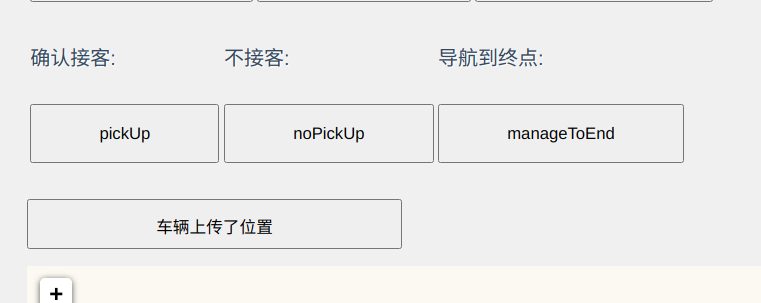
\includegraphics[width=0.8\textwidth]{images/vehicleInit.png}
    \caption{司机的初始化}\label{司机的初始化} % label 用来在文中索引
\end{figure}

此时启动\verb|passenger_test.py|,程序将启动另一个浏览器窗口操作,此时需要在司机端浏览器窗口选择接客与否:

\begin{figure}[htbp]
    \centering
    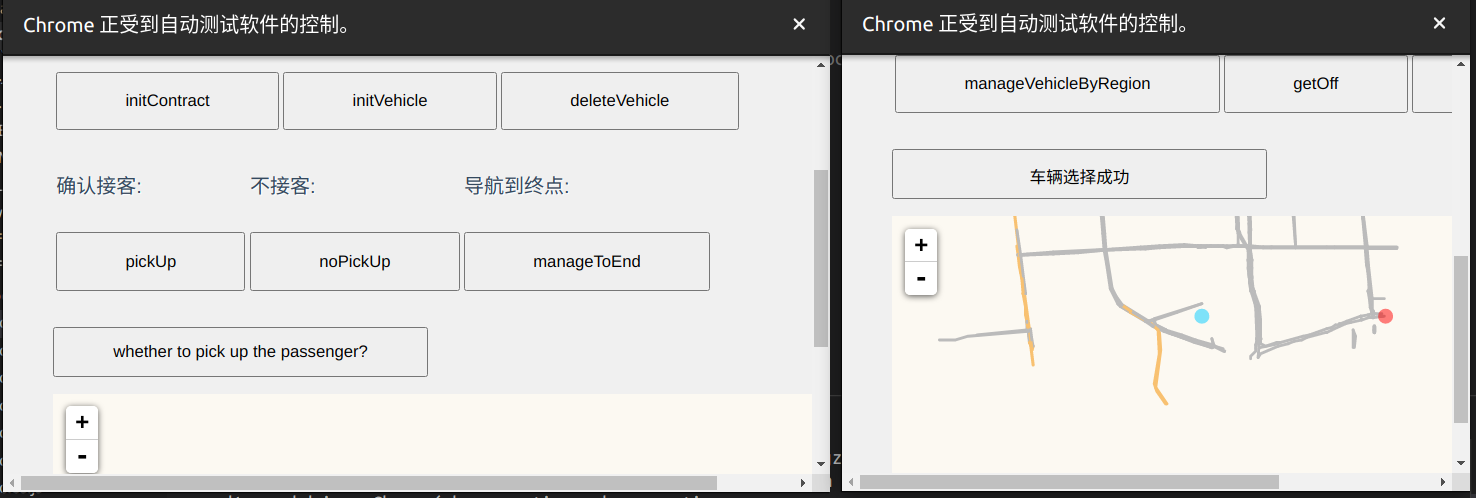
\includegraphics[width=0.8\textwidth]{images/pickUp.png}
    \caption{司机手动接客}\label{司机手动接客} % label 用来在文中索引
\end{figure}

按下pickUp按钮,程序将继续自动运行,直至看到如下输出,调度成功:

\begin{figure}[htbp]
    \centering
    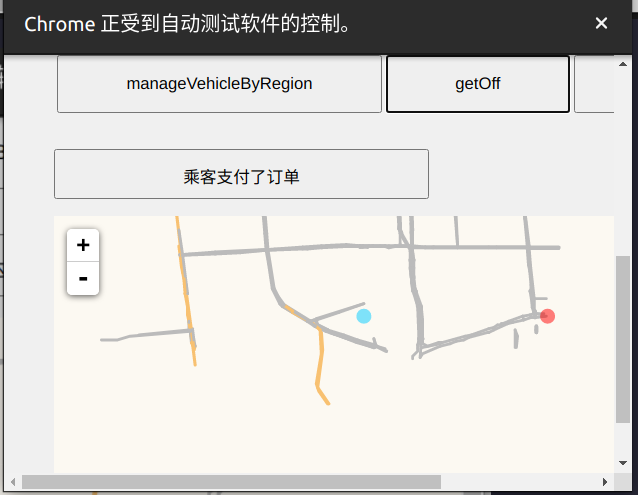
\includegraphics[width=0.8\textwidth]{images/passengerPay.png}
    \caption{乘客抵达并支付}\label{司机手动接乘客抵达并支付客} % label 用来在文中索引
\end{figure}

至此,原复现手册中的所有预期结果均已达到,调度系统复现实验全部完成。

\section{问题及解决方案}

笔者在进行出租车调度系统复现实验及其前置时,遇到许多原复现手册中未提及或未强调的注意事项;原版代码中,亦存在已废弃的语法和有待改进的设计。本节将陈述笔者遇到的问题及其解决方法。

\subsection{创世配置文件指代不明}

原复现手册中,并未指明在进行复现实验时使用的创世配置文件。经过笔者测试,附录A中的创世配置文件可用于所有出租车调度系统复现实验的全部环节。笔者已将其补充到代码仓库和新版复现手册中。

\subsection{节点无法加入区块链网络}

笔者在尝试建立双节点区块链网络时发现,无论如何使用\verb|admin.addPeer()|函数,尝试将第二个节点连接到第一个节点,都无法成功,观察\verb|net.peerCount|的值始终为0,代表着第二个节点并未发现第一个节点。

实际上,节点与区块链网络中的其他节点使用的创世配置文件完全相同,是该节点加入此区块链网络的必要条件。因此,在配置第二个节点时,必须保证两个节点的创世配置文件完全相同。

需要注意的是,创世配置文件设定了各个账户的初始信息,例如余额和初始位置等等。因此,两个节点的创世配置文件完全相同,意味着两个节点中需要存在完全一致的账号。这要求程序员将第一个节点的keystore文件夹复制到第二个节点的相同的相对路径下。

综合以上两点,可以得出结论:当节点无法加入区块链网络时,需要检查节点的创世配置文件是否相同,以及节点的keystore文件夹内的内容是否一致。同时满足以上两点条件,节点才能成功加入区块链网络。

\subsection{合约相关错误}

在浏览器的前端系统中进行操作时,按下F12打开开发者选项窗口,可能会见到有关汽油费的错误提示(Out of Gas)。经过排查,这是合约的编写、上传、调用的过程出现了错误。由于问题隐蔽、报错信息不能直接反应实际问题点,笔者花费了较多时间调试合约相关之错误。现将部署合约以及与合约交互的正确操作流程陈述如下。

\subsubsection{编译合约}

笔者使用Remix Desktop进行合约编译。编译完成后,切换到编译选项界面,点击“Compilation Details”按钮,即可观察编译结果的详细信息,如下图所示:

\begin{figure}[htbp]
    \centering
    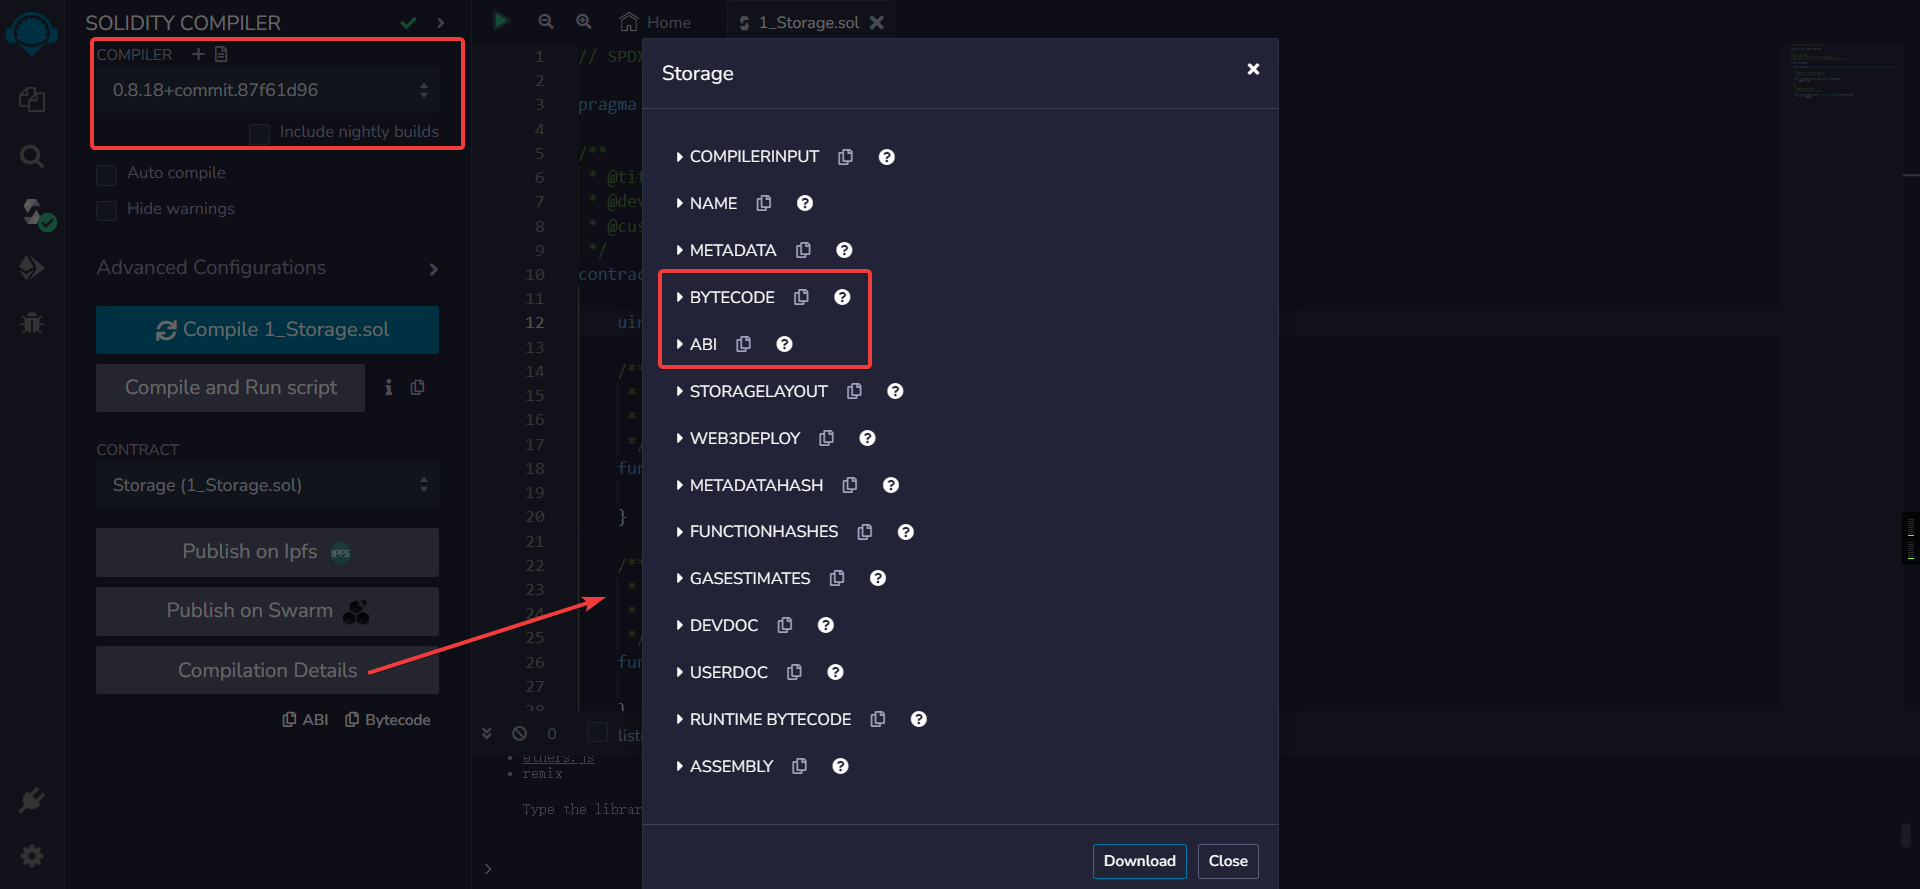
\includegraphics[width=0.8\textwidth]{images/remix.png}
    \caption{Remix IDE编译选项界面}\label{Remix IDE编译选项界面} % label 用来在文中索引
\end{figure}

图中,更靠近中央部分的红框即为部署合约时需要使用的应用程序二进制接口(ABI)和以太坊虚拟机字节码(bytecode)信息,需要妥善记录保存。另外,在合约源代码所在的目录下的artifacts目录中,有一份与合约同名的json文件,该文件亦需要妥善保存备用。

\subsubsection{部署合约}

本文使用附录B中的合约部署模板进行合约部署工作,具体步骤如下:

\begin{enumerate}
    \item 将代码模板中的“经过压缩转义后的ABI”替换为经过压缩转义处理(即:去除多余空格,且为双引号等特殊字符进行转义处理)的上一步骤中获得之应用程序二进制接口
    \item 将“获得的字节码字符串”替换为上一步骤中获得之以太坊虚拟机字节码
    \item 修改变量名Contract、contractInstance为合适的名字,避免多份合约重名
    \item 将经过以上修改的模板代码复制到正在运行geth1的控制台中,单击回车提交部署请求
    \item 使用\verb|miner.start()|开始挖矿,合约地址将随后在终端中显示
\end{enumerate}

需要注意的是,在模板中,可见一名为position的字段。若该字段指代的Geohash在区块链的管辖范围之外(即:区块链管辖的Geohash并非position字段的前缀),将获得out of the blockchain错误,无法继续部署。因此,每次部署前,均需检查position字段指示的范围是否在区块链管辖范围以内。

\subsubsection{合约交互}

部署完成后的合约可以使用合约地址与其建立交互渠道,并调用合约内定义的方法。在web3.js库的辅助下,与合约进行交互仅需短短数行代码。最小示例如下:

\begin{lstlisting}[caption={合约交互}, label={lst:合约交互}]
// 使用web3.js库
const Web3 = require('web3');
// 使用WebSocket协议连接到区块链,本例中端口号为8546
let web3 = new Web3(new Web3.providers.WebsocketProvider("ws://127.0.0.1:8546"));
// 部署合约时获得的合约地址
let contractAddress = '0x23b98f92ceac005e570b6768da377b3abd11012e';
// 编译合约时保存的应用程序二进制接口信息
let contractAbi = JSON.parse(fs.readFileSync('./contractAbi.json', 'utf-8'));
// 合约实例
let contractInstance = new web3.eth.Contract(mapContractAbi, mapContractAddress);
// 调用合约中定义的example方法
contractInstance.methods.example().then((res) => {/* 处理返回值res */});
\end{lstlisting}

在进行实验时,若出现难以排查的错误,应首先考虑合约相关错误。综合上述部署步骤,合约相关错误可以从以下几点进行排查:

\begin{itemize}
    \item 从编译详情处获得的各项数据是否正确?例如,以太坊虚拟机字节码是否与应用程序二进制接口出自同一次编译过程?
    \item 部署合约时,是否正确配置各选项,例如position字段?
    \item 部署完成之后,是否正确记录合约地址?
    \item 进行合约交互前,是否确认区块链允许WebSocket协议连接?部分功能,例如订阅事件,仅能在WebSocket连接下进行。若无,则这些功能可能失效,与合约的交互可能失败。
\end{itemize}

\section{本章小结}

本章介绍了使用区域索引区块链进行基于区块链的出租车调度系统的复现实验之相关工作。首先,简要介绍该调度系统的功能及其组成部分;其次,介绍实验进行的环境配置和包括建立区块链、部署合约、上传地图、前端调试和使用等复现步骤,并展示了复现工作的运行结果,证明了复现工作的正确性;最后,介绍了在进行复现实验时遇到的典型疑难问题,对这些问题进行了产生原因的剖析,给出了解决方法和排查思路。
